\documentclass{beamer}

%%%%%%%%%%%%%%%%%%%%%%%%%%%%%%%%%
%%% include preamble commands %%%
%%%                           %%%
%%% -makes beamer simplified  %%%
%%% -include particle symbols %%%
%%% -custom decay commands    %%%
%%%%%%%%%%%%%%%%%%%%%%%%%%%%%%%%%

%%%%%%%%%%%%%%%%%%%%%%%%%%%%%%%%%%%%%%%%%%%%%%%%%%%%%%%%%%%%%%%%%%%%%%%%%
% This is a butt-load of preamble commands to setup beamer how I like it.
% It modifies a fair amount of stuff but hopefully I've labelled 
% everything neatly and explicitly.
% 
% Sam Cunliffe May 2012
%%%%%%%%%%%%%%%%%%%%%%%%%%%%%%%%%%%%%%%%%%%%%%%%%%%%%%%%%%%%%%%%%%%%%%%%%

% use minimalist beamer template as a starting point
\usebeamertemplate{default}

%%%%%%%%%%%%%%%%%%
%%% colouring  %%%
%%%%%%%%%%%%%%%%%%

% sam's favourite blues
\definecolor{bleufonce}{RGB}{65,105,225}
\definecolor{vertfonce}{RGB}{96,189,99}
\definecolor{bleu}{RGB}{209,232,255}

% set colors
\setbeamercolor{title}{fg=black}      
\setbeamercolor{frametitle}{fg=black}
\setbeamercolor{structure}{fg=black}
\setbeamercolor{background canvas}{bg=white}%=milkyblue}

%%%%%%%%%%%%%%%%%%%%%%%%
%%% font formatting  %%%
%%%%%%%%%%%%%%%%%%%%%%%%

% a font package which has a nicer serif font
% than usual  helvet
\usepackage{charter}

% makes bulleted lists appear slightly 
% transparent before uncovering the bullet
\beamertemplatetransparentcovereddynamicmedium

% puts titles in bold
\usefonttheme{structurebold}  

% makes font serif
\usefonttheme{serif} 
\usepackage{wrapfig} 

% include and configure hyperlinks
\usepackage{hyperref}
\hypersetup{
    bookmarks=true,         % show bookmarks bar?
    %unicode=false,          % non-Latin characters in Acrobat’s bookmarks
    pdftoolbar=true,        % show Acrobat’s toolbar?
    pdfmenubar=true,        % show Acrobat’s menu?
    pdffitwindow=false,     % window fit to page when opened
    %pdfstartview={FitH},    % fits the width of the page to the window
    %pdftitle={My title},    % title
    %pdfauthor={Author},     % author
    %pdfsubject={Subject},   % subject of the document
    %pdfcreator={Creator},   % creator of the document
    %pdfproducer={Producer}, % producer of the document
    %pdfkeywords={keyword1} {key2} {key3}, % list of keywords
    %pdfnewwindow=true,      % links in new window
    colorlinks=true,       % false: boxed links; true: colored links
    linkcolor=blue,        % color of internal links
    citecolor=green,        % color of links to bibliography
    filecolor=magenta,      % color of file links
    urlcolor=blue           % color of external links
}

% allow for upright greek
\usepackage{upgreek}

% split long lists etc into two columns
\usepackage{multicol}

% les diagrams feynman
%\usepackage{axodraw}

%%%%%%%%%%%%%%%%%%%
%% table spacing %%
%%%%%%%%%%%%%%%%%%%
%\newcommand\Top{\rule{0pt}{2.6ex}}
%\newcommand\Bot{\rule[-1.2ex]{0pt}{0pt}}
\renewcommand{\arraystretch}{1.5}


%%%%%%%%%%%%%%%%%%%%%%%%%%%%%%%%%%%
%%% math and symbol formatting  %%%
%%%%%%%%%%%%%%%%%%%%%%%%%%%%%%%%%%%
\usepackage{amsmath}

% Backup with slide numbers that don't contribute to the total
\newcommand{\beginbackup}{
   \newcounter{framenumbervorappendix}
   \setcounter{framenumbervorappendix}{\value{framenumber}}
}
\newcommand{\backupend}{
   \addtocounter{framenumbervorappendix}{-\value{framenumber}}
   \addtocounter{framenumber}{\value{framenumbervorappendix}} 
}


%%%%%%%%%%%%%%%%%%%%%%%%%%%%%%%%%%%%%%%%%%
%%% slide numbering footer formatting  %%%
%%%%%%%%%%%%%%%%%%%%%%%%%%%%%%%%%%%%%%%%%%

% turns off useless semitransparent buttons
% on the bottom left hand side of all slides
% seriously, they contribute ABSOLUTELY NOTHING
\setbeamertemplate{navigation symbols}{}

% edits the template's footer
\setbeamertemplate
{footline}              %
{                       %
\color{gray}            % makes the text in the footer grey
\hspace*{1em}           % moves stuff 1em from the LHS of the page
%\,/\,                   %  linux directory type structure
%\insertsubsection       %
%\hfill                  % horizontal filling space
\insertshortauthor      % inserts author arguement in []'s
\,(\insertshortinstitute)
\hspace*{1em}           % a 1em space between author and page number
\insertshortdate
\hfill
\insertsection          % prints section name if any
\hfill
\insertframenumber/\inserttotalframenumber      % page number
\hspace*{1em}           % moves stuff 1em from the RHS of the page
% \vskip0.05cm          % moves stuff 10pts up from the bottom
\vspace*{1em}           %
} 

%%%%%%%%%%%%%%%%%%%%%%%%%%%%%%%%%%%%%%%%%%%%%%%%%%%%%%%%%%%%%%%%%%%%%%%%%
% This is a few preamble commands to set up and import all LHCb symbols
% it requires the file 'lhcb-symbols-def.tex' which should be in the 
% directory with the talk.
% 
% Sam Cunliffe May 2012
%%%%%%%%%%%%%%%%%%%%%%%%%%%%%%%%%%%%%%%%%%%%%%%%%%%%%%%%%%%%%%%%%%%%%%%%%

% some packages needed for 
% lhcb symbols definitions
\usepackage{xspace}  % sorts out spacing in and out of math mode
\usepackage{ifthen}  % allows boolean vars to control decisions

% choose how particles are displayed
\newboolean{uprightparticles}
\setboolean{uprightparticles}{false} %true == roman particle symbols

% import all lhcb symbols
%%% $Id: lhcb-symbols-def.tex 13549 2012-01-12 20:34:59Z uegede $
%%% ======================================================================
%%% Purpose: standard LHCb aliases
%%% Author: Originally Ulrik Egede, adapted by Tomasz Skwarnicki for templates,
%%% rewritten by Chris Parkes
%%% Created on: 2009-09-24
%%% =======================================================================

%%% this has to go before \begin{document}
%%%\usepackage{ifthen} 
%%%\newboolean{uprightparticles}
%%%\setboolean{uprightparticles}{true} %Set to false to get italic particle symbols

%%% Add comments with at least three %%% preceding.
%%% Add new sections with one % preceding
%%% Add new subsections with two %% preceding

%%%%%%%%%%%%%
% Experiments
%%%%%%%%%%%%%
\def\lhcb {LHCb\xspace}
\def\ux85 {UX85\xspace}
\def\cern {CERN\xspace}
\def\lhc {LHC\xspace}
\def\atlas {ATLAS\xspace}
\def\cms {CMS\xspace}
\def\babar  {BaBar\xspace}
\def\belle  {Belle\xspace}
\def\aleph  {ALEPH\xspace}
\def\delphi {DELPHI\xspace}
\def\opal   {OPAL\xspace}
\def\lthree {L3\xspace}
\def\lep    {LEP\xspace}
\def\cdf    {CDF\xspace}
\def\dzero  {D0\xspace}
\def\sld    {SLD\xspace}
\def\cleo   {CLEO\xspace}
\def\uaone  {UA1\xspace}
\def\uatwo  {UA2\xspace}
\def\tevatron {TEVATRON\xspace}

%% LHCb sub-detectors and sub-systems

\def\pu     {PU\xspace}
\def\velo   {VELO\xspace}
\def\rich   {RICH\xspace}
\def\richone {RICH1\xspace}
\def\richtwo {RICH2\xspace}
\def\ttracker {TT\xspace}
\def\intr   {IT\xspace}
\def\st     {ST\xspace}
\def\ot     {OT\xspace}
\def\Tone   {T1\xspace}
\def\Ttwo   {T2\xspace}
\def\Tthree {T3\xspace}
\def\Mone   {M1\xspace}
\def\Mtwo   {M2\xspace}
\def\Mthree {M3\xspace}
\def\Mfour  {M4\xspace}
\def\Mfive  {M5\xspace}
\def\ecal   {ECAL\xspace}
\def\spd    {SPD\xspace}
\def\presh  {PS\xspace}
\def\hcal   {HCAL\xspace}
\def\bcm    {BCM\xspace}

\def\ode    {ODE\xspace}
\def\daq    {DAQ\xspace}
\def\tfc    {TFC\xspace}
\def\ecs    {ECS\xspace}
\def\lone   {L0\xspace}
\def\hlt    {HLT\xspace}
\def\hltone {HLT1\xspace}
\def\hlttwo {HLT2\xspace}

%%% Upright (not slanted) Particles

\ifthenelse{\boolean{uprightparticles}}%
{\def\Palpha      {\ensuremath{\upalpha}\xspace}
 \def\Pbeta       {\ensuremath{\upbeta}\xspace}
 \def\Pgamma      {\ensuremath{\upgamma}\xspace}                 
 \def\Pdelta      {\ensuremath{\updelta}\xspace}                 
 \def\Pepsilon    {\ensuremath{\upepsilon}\xspace}                 
 \def\Pvarepsilon {\ensuremath{\upvarepsilon}\xspace}                 
 \def\Pzeta       {\ensuremath{\upzeta}\xspace}                 
 \def\Peta        {\ensuremath{\upeta}\xspace}                 
 \def\Ptheta      {\ensuremath{\uptheta}\xspace}                 
 \def\Pvartheta   {\ensuremath{\upvartheta}\xspace}                 
 \def\Piota       {\ensuremath{\upiota}\xspace}                 
 \def\Pkappa      {\ensuremath{\upkappa}\xspace}                 
 \def\Plambda     {\ensuremath{\uplambda}\xspace}                 
 \def\Pmu         {\ensuremath{\upmu}\xspace}                 
 \def\Pnu         {\ensuremath{\upnu}\xspace}                 
 \def\Pxi         {\ensuremath{\upxi}\xspace}                 
 \def\Ppi         {\ensuremath{\uppi}\xspace}                 
 \def\Pvarpi      {\ensuremath{\upvarpi}\xspace}                 
 \def\Prho        {\ensuremath{\uprho}\xspace}                 
 \def\Pvarrho     {\ensuremath{\upvarrho}\xspace}                 
 \def\Ptau        {\ensuremath{\uptau}\xspace}                 
 \def\Pupsilon    {\ensuremath{\upupsilon}\xspace}                 
 \def\Pphi        {\ensuremath{\upphi}\xspace}                 
 \def\Pvarphi     {\ensuremath{\upvarphi}\xspace}                 
 \def\Pchi        {\ensuremath{\upchi}\xspace}                 
 \def\Ppsi        {\ensuremath{\uppsi}\xspace}                 
 \def\Pomega      {\ensuremath{\upomega}\xspace}                 

 \def\PDelta      {\ensuremath{\Delta}\xspace}                 
 \def\PXi      {\ensuremath{\Xi}\xspace}                 
 \def\PLambda      {\ensuremath{\Lambda}\xspace}                 
 \def\PSigma      {\ensuremath{\Sigma}\xspace}                 
 \def\POmega      {\ensuremath{\Omega}\xspace}                 
 \def\PUpsilon      {\ensuremath{\Upsilon}\xspace}                 
 
 %\mathchardef\Deltares="7101
 %\mathchardef\Xi="7104
 %\mathchardef\Lambda="7103
 %\mathchardef\Sigma="7106
 %\mathchardef\Omega="710A


 \def\PA      {\ensuremath{\mathrm{A}}\xspace}                 
 \def\PB      {\ensuremath{\mathrm{B}}\xspace}                 
 \def\PC      {\ensuremath{\mathrm{C}}\xspace}                 
 \def\PD      {\ensuremath{\mathrm{D}}\xspace}                 
 \def\PE      {\ensuremath{\mathrm{E}}\xspace}                 
 \def\PF      {\ensuremath{\mathrm{F}}\xspace}                 
 \def\PG      {\ensuremath{\mathrm{G}}\xspace}                 
 \def\PH      {\ensuremath{\mathrm{H}}\xspace}                 
 \def\PI      {\ensuremath{\mathrm{I}}\xspace}                 
 \def\PJ      {\ensuremath{\mathrm{J}}\xspace}                 
 \def\PK      {\ensuremath{\mathrm{K}}\xspace}                 
 \def\PL      {\ensuremath{\mathrm{L}}\xspace}                 
 \def\PM      {\ensuremath{\mathrm{M}}\xspace}                 
 \def\PN      {\ensuremath{\mathrm{N}}\xspace}                 
 \def\PO      {\ensuremath{\mathrm{O}}\xspace}                 
 \def\PP      {\ensuremath{\mathrm{P}}\xspace}                 
 \def\PQ      {\ensuremath{\mathrm{Q}}\xspace}                 
 \def\PR      {\ensuremath{\mathrm{R}}\xspace}                 
 \def\PS      {\ensuremath{\mathrm{S}}\xspace}                 
 \def\PT      {\ensuremath{\mathrm{T}}\xspace}                 
 \def\PU      {\ensuremath{\mathrm{U}}\xspace}                 
 \def\PV      {\ensuremath{\mathrm{V}}\xspace}                 
 \def\PW      {\ensuremath{\mathrm{W}}\xspace}                 
 \def\PX      {\ensuremath{\mathrm{X}}\xspace}                 
 \def\PY      {\ensuremath{\mathrm{Y}}\xspace}                 
 \def\PZ      {\ensuremath{\mathrm{Z}}\xspace}                 
 \def\Pa      {\ensuremath{\mathrm{a}}\xspace}                 
 \def\Pb      {\ensuremath{\mathrm{b}}\xspace}                 
 \def\Pc      {\ensuremath{\mathrm{c}}\xspace}                 
 \def\Pd      {\ensuremath{\mathrm{d}}\xspace}                 
 \def\Pe      {\ensuremath{\mathrm{e}}\xspace}                 
 \def\Pf      {\ensuremath{\mathrm{f}}\xspace}                 
 \def\Pg      {\ensuremath{\mathrm{g}}\xspace}                 
 \def\Ph      {\ensuremath{\mathrm{h}}\xspace}                 
 \def\Pi      {\ensuremath{\mathrm{i}}\xspace}                 
 \def\Pj      {\ensuremath{\mathrm{j}}\xspace}                 
 \def\Pk      {\ensuremath{\mathrm{k}}\xspace}                 
 \def\Pl      {\ensuremath{\mathrm{l}}\xspace}                 
 \def\Pm      {\ensuremath{\mathrm{m}}\xspace}                 
 \def\Pn      {\ensuremath{\mathrm{n}}\xspace}                 
 \def\Po      {\ensuremath{\mathrm{o}}\xspace}                 
 \def\Pp      {\ensuremath{\mathrm{p}}\xspace}                 
 \def\Pq      {\ensuremath{\mathrm{q}}\xspace}                 
 \def\Pr      {\ensuremath{\mathrm{r}}\xspace}                 
 \def\Ps      {\ensuremath{\mathrm{s}}\xspace}                 
 \def\Pt      {\ensuremath{\mathrm{t}}\xspace}                 
 \def\Pu      {\ensuremath{\mathrm{u}}\xspace}                 
 \def\Pv      {\ensuremath{\mathrm{v}}\xspace}                 
 \def\Pw      {\ensuremath{\mathrm{w}}\xspace}                 
 \def\Px      {\ensuremath{\mathrm{x}}\xspace}                 
 \def\Py      {\ensuremath{\mathrm{y}}\xspace}                 
 \def\Pz      {\ensuremath{\mathrm{z}}\xspace}                 
}
{\def\Palpha      {\ensuremath{\alpha}\xspace}
 \def\Pbeta       {\ensuremath{\beta}\xspace}
 \def\Pgamma      {\ensuremath{\gamma}\xspace}                 
 \def\Pdelta      {\ensuremath{\delta}\xspace}                 
 \def\Pepsilon    {\ensuremath{\epsilon}\xspace}                 
 \def\Pvarepsilon {\ensuremath{\varepsilon}\xspace}                 
 \def\Pzeta       {\ensuremath{\zeta}\xspace}                 
 \def\Peta        {\ensuremath{\eta}\xspace}                 
 \def\Ptheta      {\ensuremath{\theta}\xspace}                 
 \def\Pvartheta   {\ensuremath{\vartheta}\xspace}                 
 \def\Piota       {\ensuremath{\iota}\xspace}                 
 \def\Pkappa      {\ensuremath{\kappa}\xspace}                 
 \def\Plambda     {\ensuremath{\lambda}\xspace}                 
 \def\Pmu         {\ensuremath{\mu}\xspace}                 
 \def\Pnu         {\ensuremath{\nu}\xspace}                 
 \def\Pxi         {\ensuremath{\xi}\xspace}                 
 \def\Ppi         {\ensuremath{\pi}\xspace}                 
 \def\Pvarpi      {\ensuremath{\varpi}\xspace}                 
 \def\Prho        {\ensuremath{\rho}\xspace}                 
 \def\Pvarrho     {\ensuremath{\varrho}\xspace}                 
 \def\Ptau        {\ensuremath{\tau}\xspace}                 
 \def\Pupsilon    {\ensuremath{\upsilon}\xspace}                 
 \def\Pphi        {\ensuremath{\phi}\xspace}                 
 \def\Pvarphi     {\ensuremath{\varphi}\xspace}                 
 \def\Pchi        {\ensuremath{\chi}\xspace}                 
 \def\Ppsi        {\ensuremath{\psi}\xspace}                 
 \def\Pomega      {\ensuremath{\omega}\xspace}                 
 \mathchardef\PDelta="7101
 \mathchardef\PXi="7104
 \mathchardef\PLambda="7103
 \mathchardef\PSigma="7106
 \mathchardef\POmega="710A
 \mathchardef\PUpsilon="7107
 \def\PA      {\ensuremath{A}\xspace}                 
 \def\PB      {\ensuremath{B}\xspace}                 
 \def\PC      {\ensuremath{C}\xspace}                 
 \def\PD      {\ensuremath{D}\xspace}                 
 \def\PE      {\ensuremath{E}\xspace}                 
 \def\PF      {\ensuremath{F}\xspace}                 
 \def\PG      {\ensuremath{G}\xspace}                 
 \def\PH      {\ensuremath{H}\xspace}                 
 \def\PI      {\ensuremath{I}\xspace}                 
 \def\PJ      {\ensuremath{J}\xspace}                 
 \def\PK      {\ensuremath{K}\xspace}                 
 \def\PL      {\ensuremath{L}\xspace}                 
 \def\PM      {\ensuremath{M}\xspace}                 
 \def\PN      {\ensuremath{N}\xspace}                 
 \def\PO      {\ensuremath{O}\xspace}                 
 \def\PP      {\ensuremath{P}\xspace}                 
 \def\PQ      {\ensuremath{Q}\xspace}                 
 \def\PR      {\ensuremath{R}\xspace}                 
 \def\PS      {\ensuremath{S}\xspace}                 
 \def\PT      {\ensuremath{T}\xspace}                 
 \def\PU      {\ensuremath{U}\xspace}                 
 \def\PV      {\ensuremath{V}\xspace}                 
 \def\PW      {\ensuremath{W}\xspace}                 
 \def\PX      {\ensuremath{X}\xspace}                 
 \def\PY      {\ensuremath{Y}\xspace}                 
 \def\PZ      {\ensuremath{Z}\xspace}                 
 \def\Pa      {\ensuremath{a}\xspace}                 
 \def\Pb      {\ensuremath{b}\xspace}                 
 \def\Pc      {\ensuremath{c}\xspace}                 
 \def\Pd      {\ensuremath{d}\xspace}                 
 \def\Pe      {\ensuremath{e}\xspace}                 
 \def\Pf      {\ensuremath{f}\xspace}                 
 \def\Pg      {\ensuremath{g}\xspace}                 
 \def\Ph      {\ensuremath{h}\xspace}                 
 \def\Pi      {\ensuremath{i}\xspace}                 
 \def\Pj      {\ensuremath{j}\xspace}                 
 \def\Pk      {\ensuremath{k}\xspace}                 
 \def\Pl      {\ensuremath{l}\xspace}                 
 \def\Pm      {\ensuremath{m}\xspace}                 
 \def\Pn      {\ensuremath{n}\xspace}                 
 \def\Po      {\ensuremath{o}\xspace}                 
 \def\Pp      {\ensuremath{p}\xspace}                 
 \def\Pq      {\ensuremath{q}\xspace}                 
 \def\Pr      {\ensuremath{r}\xspace}                 
 \def\Ps      {\ensuremath{s}\xspace}                 
 \def\Pt      {\ensuremath{t}\xspace}                 
 \def\Pu      {\ensuremath{u}\xspace}                 
 \def\Pv      {\ensuremath{v}\xspace}                 
 \def\Pw      {\ensuremath{w}\xspace}                 
 \def\Px      {\ensuremath{x}\xspace}                 
 \def\Py      {\ensuremath{y}\xspace}                 
 \def\Pz      {\ensuremath{z}\xspace}                 
}

%%%%%%%%%%%%%%%%%%%%%%%%%%%%%%%%%%%%%%%%%%%%%%%
% Particles

%% Leptons

\let\emi\en
\def\electron   {\ensuremath{\Pe}\xspace}
\def\en         {\ensuremath{\Pe^-}\xspace}   % electron negative (\em is taken)
\def\ep         {\ensuremath{\Pe^+}\xspace}
\def\epm        {\ensuremath{\Pe^\pm}\xspace} 
\def\epem       {\ensuremath{\Pe^+\Pe^-}\xspace}
\def\ee         {\ensuremath{\Pe^-\Pe^-}\xspace}

\def\mmu        {\ensuremath{\Pmu}\xspace}
\def\mup        {\ensuremath{\Pmu^+}\xspace}
\def\mun        {\ensuremath{\Pmu^-}\xspace} % muon negative (\mum is taken)
\def\mumu       {\ensuremath{\Pmu^+\Pmu^-}\xspace}
\def\mtau       {\ensuremath{\Ptau}\xspace}

\def\taup       {\ensuremath{\Ptau^+}\xspace}
\def\taum       {\ensuremath{\Ptau^-}\xspace}
\def\tautau     {\ensuremath{\Ptau^+\Ptau^-}\xspace}

\def\ellm       {\ensuremath{\ell^-}\xspace}
\def\ellp       {\ensuremath{\ell^+}\xspace}
\def\ellell     {\ensuremath{\ell^+ \ell^-}\xspace}

\def\neu        {\ensuremath{\Pnu}\xspace}
\def\neub       {\ensuremath{\overline{\Pnu}}\xspace}
\def\nuenueb    {\ensuremath{\neu\neub}\xspace}
\def\neue       {\ensuremath{\neu_e}\xspace}
\def\neueb      {\ensuremath{\neub_e}\xspace}
\def\neueneueb  {\ensuremath{\neue\neueb}\xspace}
\def\neum       {\ensuremath{\neu_\mu}\xspace}
\def\neumb      {\ensuremath{\neub_\mu}\xspace}
\def\neumneumb  {\ensuremath{\neum\neumb}\xspace}
\def\neut       {\ensuremath{\neu_\tau}\xspace}
\def\neutb      {\ensuremath{\neub_\tau}\xspace}
\def\neutneutb  {\ensuremath{\neut\neutb}\xspace}
\def\neul       {\ensuremath{\neu_\ell}\xspace}
\def\neulb      {\ensuremath{\neub_\ell}\xspace}
\def\neulneulb  {\ensuremath{\neul\neulb}\xspace}

%% Gauge bosons and scalars

\def\g      {\ensuremath{\Pgamma}\xspace}
\def\H      {\ensuremath{\PH^0}\xspace}
\def\Hp     {\ensuremath{\PH^+}\xspace}
\def\Hm     {\ensuremath{\PH^-}\xspace}
\def\Hpm    {\ensuremath{\PH^\pm}\xspace}
\def\W      {\ensuremath{\PW}\xspace}
\def\Wp     {\ensuremath{\PW^+}\xspace}
\def\Wm     {\ensuremath{\PW^-}\xspace}
\def\Wpm    {\ensuremath{\PW^\pm}\xspace}
\def\Z      {\ensuremath{\PZ^0}\xspace}

%% Quarks

\def\quark     {\ensuremath{\Pq}\xspace}
\def\quarkbar  {\ensuremath{\overline \quark}\xspace}
\def\qqbar     {\ensuremath{\quark\quarkbar}\xspace}
\def\uquark    {\ensuremath{\Pu}\xspace}
\def\uquarkbar {\ensuremath{\overline \uquark}\xspace}
\def\uubar     {\ensuremath{\uquark\uquarkbar}\xspace}
\def\dquark    {\ensuremath{\Pd}\xspace}
\def\dquarkbar {\ensuremath{\overline \dquark}\xspace}
\def\ddbar     {\ensuremath{\dquark\dquarkbar}\xspace}
\def\squark    {\ensuremath{\Ps}\xspace}
\def\squarkbar {\ensuremath{\overline \squark}\xspace}
\def\ssbar     {\ensuremath{\squark\squarkbar}\xspace}
\def\cquark    {\ensuremath{\Pc}\xspace}
\def\cquarkbar {\ensuremath{\overline \cquark}\xspace}
\def\ccbar     {\ensuremath{\cquark\cquarkbar}\xspace}
\def\bquark    {\ensuremath{\Pb}\xspace}
\def\bquarkbar {\ensuremath{\overline \bquark}\xspace}
\def\bbbar     {\ensuremath{\bquark\bquarkbar}\xspace}
\def\tquark    {\ensuremath{\Pt}\xspace}
\def\tquarkbar {\ensuremath{\overline \tquark}\xspace}
\def\ttbar     {\ensuremath{\tquark\tquarkbar}\xspace}

%% Light mesons

\def\pion  {\ensuremath{\Ppi}\xspace}
\def\piz   {\ensuremath{\pion^0}\xspace}
\def\pizs  {\ensuremath{\pion^0\mbox\,\rm{s}}\xspace}
\def\ppz   {\ensuremath{\pion^0\pion^0}\xspace}
\def\pip   {\ensuremath{\pion^+}\xspace}
\def\pim   {\ensuremath{\pion^-}\xspace}
\def\pipi  {\ensuremath{\pion^+\pion^-}\xspace}
\def\pipm  {\ensuremath{\pion^\pm}\xspace}
\def\pimp  {\ensuremath{\pion^\mp}\xspace}

\def\kaon  {\ensuremath{\PK}\xspace}
%%% do NOT use ensuremath here
  \def\Kbar  {\kern 0.2em\overline{\kern -0.2em \PK}{}\xspace}
\def\Kb    {\ensuremath{\Kbar}\xspace}
\def\Kz    {\ensuremath{\kaon^0}\xspace}
\def\Kzb   {\ensuremath{\Kbar^0}\xspace}
\def\KzKzb {\ensuremath{\Kz \kern -0.16em \Kzb}\xspace}
\def\Kp    {\ensuremath{\kaon^+}\xspace}
\def\Km    {\ensuremath{\kaon^-}\xspace}
\def\Kpm   {\ensuremath{\kaon^\pm}\xspace}
\def\Kmp   {\ensuremath{\kaon^\mp}\xspace}
\def\KpKm  {\ensuremath{\Kp \kern -0.16em \Km}\xspace}
\def\KS    {\ensuremath{\kaon^0_{\rm\scriptscriptstyle S}}\xspace} 
\def\KL    {\ensuremath{\kaon^0_{\rm\scriptscriptstyle L}}\xspace} 
\def\Kstarz  {\ensuremath{\kaon^{*0}}\xspace}
\def\Kstarzb {\ensuremath{\Kbar^{*0}}\xspace}
\def\Kstar   {\ensuremath{\kaon^*}\xspace}
\def\Kstarb  {\ensuremath{\Kbar^*}\xspace}
\def\Kstarp  {\ensuremath{\kaon^{*+}}\xspace}
\def\Kstarm  {\ensuremath{\kaon^{*-}}\xspace}
\def\Kstarpm {\ensuremath{\kaon^{*\pm}}\xspace}
\def\Kstarmp {\ensuremath{\kaon^{*\mp}}\xspace}

\newcommand{\etapr}{\ensuremath{\Peta^{\prime}}\xspace}

%% Heavy mesons

%%% do NOT use ensuremath here
  \def\Dbar    {\kern 0.2em\overline{\kern -0.2em \PD}{}\xspace}
\def\D       {\ensuremath{\PD}\xspace}
\def\Db      {\ensuremath{\Dbar}\xspace}
\def\Dz      {\ensuremath{\D^0}\xspace}
\def\Dzb     {\ensuremath{\Dbar^0}\xspace}
\def\DzDzb   {\ensuremath{\Dz {\kern -0.16em \Dzb}}\xspace}
\def\Dp      {\ensuremath{\D^+}\xspace}
\def\Dm      {\ensuremath{\D^-}\xspace}
\def\Dpm     {\ensuremath{\D^\pm}\xspace}
\def\Dmp     {\ensuremath{\D^\mp}\xspace}
\def\DpDm    {\ensuremath{\Dp {\kern -0.16em \Dm}}\xspace}
\def\Dstar   {\ensuremath{\D^*}\xspace}
\def\Dstarb  {\ensuremath{\Dbar^*}\xspace}
\def\Dstarz  {\ensuremath{\D^{*0}}\xspace}
\def\Dstarzb {\ensuremath{\Dbar^{*0}}\xspace}
\def\Dstarp  {\ensuremath{\D^{*+}}\xspace}
\def\Dstarm  {\ensuremath{\D^{*-}}\xspace}
\def\Dstarpm {\ensuremath{\D^{*\pm}}\xspace}
\def\Dstarmp {\ensuremath{\D^{*\mp}}\xspace}
\def\Ds      {\ensuremath{\D^+_\squark}\xspace}
\def\Dsp     {\ensuremath{\D^+_\squark}\xspace}
\def\Dsm     {\ensuremath{\D^-_\squark}\xspace}
\def\Dspm    {\ensuremath{\D^{\pm}_\squark}\xspace}
\def\Dss     {\ensuremath{\D^{*+}_\squark}\xspace}
\def\Dssp    {\ensuremath{\D^{*+}_\squark}\xspace}
\def\Dssm    {\ensuremath{\D^{*-}_\squark}\xspace}
\def\Dsspm   {\ensuremath{\D^{*\pm}_\squark}\xspace}

\def\B       {\ensuremath{\PB}\xspace}
%%% do NOT use ensuremath here
  \def\Bbar    {\kern 0.18em\overline{\kern -0.18em \PB}{}\xspace}
\def\Bb      {\ensuremath{\Bbar}\xspace}
\def\BBbar   {\ensuremath{\B\Bbar}\xspace} 
\def\Bz      {\ensuremath{\B^0}\xspace}
\def\Bzb     {\ensuremath{\Bbar^0}\xspace}
\def\Bu      {\ensuremath{\B^+}\xspace}
\def\Bub     {\ensuremath{\B^-}\xspace}
\def\Bp      {\ensuremath{\Bu}\xspace}
\def\Bm      {\ensuremath{\Bub}\xspace}
\def\Bpm     {\ensuremath{\B^\pm}\xspace}
\def\Bmp     {\ensuremath{\B^\mp}\xspace}
\def\Bd      {\ensuremath{\B^0}\xspace}
\def\Bs      {\ensuremath{\B^0_\squark}\xspace}
\def\Bsb     {\ensuremath{\Bbar^0_\squark}\xspace}
\def\Bdb     {\ensuremath{\Bbar^0}\xspace}
\def\Bc      {\ensuremath{\B_\cquark^+}\xspace}
\def\Bcp     {\ensuremath{\B_\cquark^+}\xspace}
\def\Bcm     {\ensuremath{\B_\cquark^-}\xspace}
\def\Bcpm    {\ensuremath{\B_\cquark^\pm}\xspace}

%% Onia

\def\jpsi     {\ensuremath{{\PJ\mskip -3mu/\mskip -2mu\Ppsi\mskip 2mu}}\xspace}
\def\psitwos  {\ensuremath{\Ppsi{(2S)}}\xspace}
\def\psiprpr  {\ensuremath{\Ppsi(3770)}\xspace}
\def\etac     {\ensuremath{\Peta_\cquark}\xspace}
\def\chiczero {\ensuremath{\Pchi_{\cquark 0}}\xspace}
\def\chicone  {\ensuremath{\Pchi_{\cquark 1}}\xspace}
\def\chictwo  {\ensuremath{\Pchi_{\cquark 2}}\xspace}
  %\mathchardef\Upsilon="7107
  \def\Y#1S{\ensuremath{\PUpsilon{(#1S)}}\xspace}% no space before {...}!
\def\OneS  {\Y1S}
\def\TwoS  {\Y2S}
\def\ThreeS{\Y3S}
\def\FourS {\Y4S}
\def\FiveS {\Y5S}

\def\chic  {\ensuremath{\Pchi_{c}}\xspace}

%% Baryons

\def\proton      {\ensuremath{\Pp}\xspace}
\def\antiproton  {\ensuremath{\overline \proton}\xspace}
\def\neutron     {\ensuremath{\Pn}\xspace}
\def\antineutron {\ensuremath{\overline \neutron}\xspace}

\def\Deltares {\ensuremath{\PDelta}\xspace}
\def\Deltaresbar{\ensuremath{\overline \Deltares}\xspace}
\def\Xires {\ensuremath{\PXi}\xspace}
\def\Xiresbar{\ensuremath{\overline \Xires}\xspace}
\def\L {\ensuremath{\PLambda}\xspace}
\def\Lbar{\ensuremath{\overline \L}\xspace}
\def\Lambdares {\ensuremath{\PLambda}\xspace}
\def\Lambdaresbar{\ensuremath{\overline \Lambdares}\xspace}
\def\Sigmares {\ensuremath{\PSigma}\xspace}
\def\Sigmaresbar{\ensuremath{\overline \Sigmares}\xspace}
\def\Omegares {\ensuremath{\POmega}\xspace}
\def\Omegaresbar{\ensuremath{\overline \Omegares}\xspace}

%%% do NOT use ensuremath here
 % \def\Deltabar{\kern 0.25em\overline{\kern -0.25em \Deltares}{}\xspace}
 % \def\Lbar{\kern 0.2em\overline{\kern -0.2em\Lambda\kern 0.05em}\kern-0.05em{}\xspace}
 % \def\Sigbar{\kern 0.2em\overline{\kern -0.2em \Sigma}{}\xspace}
 % \def\Xibar{\kern 0.2em\overline{\kern -0.2em \Xi}{}\xspace}
 % \def\Obar{\kern 0.2em\overline{\kern -0.2em \Omega}{}\xspace}
 % \def\Nbar{\kern 0.2em\overline{\kern -0.2em N}{}\xspace}
 % \def\Xb{\kern 0.2em\overline{\kern -0.2em X}{}\xspace}

\def\Lb      {\ensuremath{\L_\bquark}\xspace}
\def\Lbbar   {\ensuremath{\Lbar_\bquark}\xspace}
\def\Lc      {\ensuremath{\L_\cquark}\xspace}
\def\Lcbar   {\ensuremath{\Lbar_\cquark}\xspace}

%%%%%%%%%%%%%%%%%%
% Physics symbols
%%%%%%%%%%%%%%%%%

%% Decays
\def\BF         {{\ensuremath{\cal B}\xspace}}
\def\BRvis      {{\ensuremath{\BR_{\rm{vis}}}}}
\def\BR         {\BF}
\newcommand{\decay}[2]{\ensuremath{#1\!\to #2}\xspace}         % {\Pa}{\Pb \Pc}
\def\ra                 {\ensuremath{\rightarrow}\xspace}
\def\to                 {\ensuremath{\rightarrow}\xspace}

%% Lifetimes
\newcommand{\tauBs}{\ensuremath{\tau_{\Bs}}\xspace}
\newcommand{\tauBd}{\ensuremath{\tau_{\Bd}}\xspace}
\newcommand{\tauBz}{\ensuremath{\tau_{\Bz}}\xspace}
\newcommand{\tauBu}{\ensuremath{\tau_{\Bp}}\xspace}
\newcommand{\tauDp}{\ensuremath{\tau_{\Dp}}\xspace}
\newcommand{\tauDz}{\ensuremath{\tau_{\Dz}}\xspace}
\newcommand{\tauL}{\ensuremath{\tau_{\rm L}}\xspace}
\newcommand{\tauH}{\ensuremath{\tau_{\rm H}}\xspace}

%% Masses
\newcommand{\mBd}{\ensuremath{m_{\Bd}}\xspace}
\newcommand{\mBp}{\ensuremath{m_{\Bp}}\xspace}
\newcommand{\mBs}{\ensuremath{m_{\Bs}}\xspace}
\newcommand{\mBc}{\ensuremath{m_{\Bc}}\xspace}
\newcommand{\mLb}{\ensuremath{m_{\Lb}}\xspace}

%% EW theory, groups
\def\grpsuthree {\ensuremath{\mathrm{SU}(3)}\xspace}
\def\grpsutw    {\ensuremath{\mathrm{SU}(2)}\xspace}
\def\grpuone    {\ensuremath{\mathrm{U}(1)}\xspace}

\def\ssqtw {\ensuremath{\sin^{2}\!\theta_{\mathrm{W}}}\xspace}
\def\csqtw {\ensuremath{\cos^{2}\!\theta_{\mathrm{W}}}\xspace}
\def\stw   {\ensuremath{\sin\theta_{\mathrm{W}}}\xspace}
\def\ctw   {\ensuremath{\cos\theta_{\mathrm{W}}}\xspace}
\def\ssqtwef {\ensuremath{{\sin}^{2}\theta_{\mathrm{W}}^{\mathrm{eff}}}\xspace}
\def\csqtwef {\ensuremath{{\cos}^{2}\theta_{\mathrm{W}}^{\mathrm{eff}}}\xspace}
\def\stwef {\ensuremath{\sin\theta_{\mathrm{W}}^{\mathrm{eff}}}\xspace}
\def\ctwef {\ensuremath{\cos\theta_{\mathrm{W}}^{\mathrm{eff}}}\xspace}
\def\gv    {\ensuremath{g_{\mbox{\tiny V}}}\xspace}
\def\ga    {\ensuremath{g_{\mbox{\tiny A}}}\xspace}

\def\order   {\ensuremath{\mathcal{O}}\xspace}
\def\ordalph {\ensuremath{\mathcal{O}(\alpha)}\xspace}
\def\ordalsq {\ensuremath{\mathcal{O}(\alpha^{2})}\xspace}
\def\ordalcb {\ensuremath{\mathcal{O}(\alpha^{3})}\xspace}

%% QCD parameters
\newcommand{\as}{\ensuremath{\alpha_{\scriptscriptstyle S}}\xspace}
\newcommand{\MSb}{\ensuremath{\overline{\mathrm{MS}}}\xspace}
\newcommand{\lqcd}{\ensuremath{\Lambda_{\mathrm{QCD}}}\xspace}
\def\qsq       {\ensuremath{q^2}\xspace}

%% CKM, CP violation

\def\eps   {\ensuremath{\varepsilon}\xspace}
\def\epsK  {\ensuremath{\varepsilon_K}\xspace}
\def\epsB  {\ensuremath{\varepsilon_B}\xspace}
\def\epsp  {\ensuremath{\varepsilon^\prime_K}\xspace}

\def\CP                {\ensuremath{C\!P}\xspace}
\def\CPT               {\ensuremath{C\!PT}\xspace}

\def\rhobar {\ensuremath{\overline \rho}\xspace}
\def\etabar {\ensuremath{\overline \eta}\xspace}

\def\Vud  {\ensuremath{|V_{\uquark\dquark}|}\xspace}
\def\Vcd  {\ensuremath{|V_{\cquark\dquark}|}\xspace}
\def\Vtd  {\ensuremath{|V_{\tquark\dquark}|}\xspace}
\def\Vus  {\ensuremath{|V_{\uquark\squark}|}\xspace}
\def\Vcs  {\ensuremath{|V_{\cquark\squark}|}\xspace}
\def\Vts  {\ensuremath{|V_{\tquark\squark}|}\xspace}
\def\Vub  {\ensuremath{|V_{\uquark\bquark}|}\xspace}
\def\Vcb  {\ensuremath{|V_{\cquark\bquark}|}\xspace}
\def\Vtb  {\ensuremath{|V_{\tquark\bquark}|}\xspace}

%% Oscillations

\newcommand{\dm}{\ensuremath{\Delta m}\xspace}
\newcommand{\dms}{\ensuremath{\Delta m_{\squark}}\xspace}
\newcommand{\dmd}{\ensuremath{\Delta m_{\dquark}}\xspace}
\newcommand{\DG}{\ensuremath{\Delta\Gamma}\xspace}
\newcommand{\DGs}{\ensuremath{\Delta\Gamma_{\squark}}\xspace}
\newcommand{\DGd}{\ensuremath{\Delta\Gamma_{\dquark}}\xspace}
\newcommand{\Gs}{\ensuremath{\Gamma_{\squark}}\xspace}
\newcommand{\Gd}{\ensuremath{\Gamma_{\dquark}}\xspace}

\newcommand{\MBq}{\ensuremath{M_{\B_\quark}}\xspace}
\newcommand{\DGq}{\ensuremath{\Delta\Gamma_{\quark}}\xspace}
\newcommand{\Gq}{\ensuremath{\Gamma_{\quark}}\xspace}
\newcommand{\dmq}{\ensuremath{\Delta m_{\quark}}\xspace}
\newcommand{\GL}{\ensuremath{\Gamma_{\rm L}}\xspace}
\newcommand{\GH}{\ensuremath{\Gamma_{\rm H}}\xspace}

\newcommand{\DGsGs}{\ensuremath{\Delta\Gamma_{\squark}/\Gamma_{\squark}}\xspace}
\newcommand{\Delm}{\mbox{$\Delta m $}\xspace}
\newcommand{\ACP}{\ensuremath{{\cal A}^{\CP}}\xspace}
\newcommand{\Adir}{\ensuremath{{\cal A}^{\rm dir}}\xspace}
\newcommand{\Amix}{\ensuremath{{\cal A}^{\rm mix}}\xspace}
\newcommand{\ADelta}{\ensuremath{{\cal A}^\Delta}\xspace}
\newcommand{\phid}{\ensuremath{\phi_{\dquark}}\xspace}
\newcommand{\sinphid}{\ensuremath{\sin\!\phid}\xspace}
\newcommand{\phis}{\ensuremath{\phi_{\squark}}\xspace}
\newcommand{\betas}{\ensuremath{\beta_{\squark}}\xspace}
\newcommand{\sbetas}{\ensuremath{\sigma(\beta_{\squark})}\xspace}
\newcommand{\stbetas}{\ensuremath{\sigma(2\beta_{\squark})}\xspace}
\newcommand{\stphis}{\ensuremath{\sigma(\phi_{\squark})}\xspace}
\newcommand{\sinphis}{\ensuremath{\sin\!\phis}\xspace}

%% Tagging
\newcommand{\edet}{{\ensuremath{\varepsilon_{\rm det}}}\xspace}
\newcommand{\erec}{{\ensuremath{\varepsilon_{\rm rec/det}}}\xspace}
\newcommand{\esel}{{\ensuremath{\varepsilon_{\rm sel/rec}}}\xspace}
\newcommand{\etrg}{{\ensuremath{\varepsilon_{\rm trg/sel}}}\xspace}
\newcommand{\etot}{{\ensuremath{\varepsilon_{\rm tot}}}\xspace}

\newcommand{\mistag}{\ensuremath{\omega}\xspace}
\newcommand{\wcomb}{\ensuremath{\omega^{\rm comb}}\xspace}
\newcommand{\etag}{{\ensuremath{\varepsilon_{\rm tag}}}\xspace}
\newcommand{\etagcomb}{{\ensuremath{\varepsilon_{\rm tag}^{\rm comb}}}\xspace}
\newcommand{\effeff}{\ensuremath{\varepsilon_{\rm eff}}\xspace}
\newcommand{\effeffcomb}{\ensuremath{\varepsilon_{\rm eff}^{\rm comb}}\xspace}
\newcommand{\efftag}{{\ensuremath{\etag(1-2\omega)^2}}\xspace}
\newcommand{\effD}{{\ensuremath{\etag D^2}}\xspace}

\newcommand{\etagprompt}{{\ensuremath{\varepsilon_{\rm tag}^{\rm Pr}}}\xspace}
\newcommand{\etagLL}{{\ensuremath{\varepsilon_{\rm tag}^{\rm LL}}}\xspace}

%% Key decay channels

\def\BdToKstmm    {\decay{\Bd}{\Kstarz\mup\mun}}
\def\BdbToKstmm   {\decay{\Bdb}{\Kstarzb\mup\mun}}

\def\BsToJPsiPhi  {\decay{\Bs}{\jpsi\phi}}
\def\BdToJPsiKst  {\decay{\Bd}{\jpsi\Kstarz}}
\def\BdbToJPsiKst {\decay{\Bdb}{\jpsi\Kstarzb}}

\def\BsPhiGam     {\decay{\Bd}{\phi \g}}
\def\BdKstGam     {\decay{\Bd}{\Kstarz \g}}

\def\BTohh        {\decay{\B}{\Ph^+ \Ph'^-}}
\def\BdTopipi     {\decay{\Bd}{\pip\pim}}
\def\BdToKpi      {\decay{\Bd}{\Kp\pim}}
\def\BsToKK       {\decay{\Bs}{\Kp\Km}}
\def\BsTopiK      {\decay{\Bs}{\pip\Km}}

%% Rare decays
\def\BdKstee  {\decay{\Bd}{\Kstarz\epem}}
\def\BdbKstee {\decay{\Bdb}{\Kstarzb\epem}}
\def\bsll     {\decay{\bquark}{\squark \ell^+ \ell^-}}
\def\AFB      {\ensuremath{A_{\mathrm{FB}}}\xspace}
\def\FL       {\ensuremath{F_{\mathrm{L}}}\xspace}
\def\AT#1     {\ensuremath{A_{\mathrm{T}}^{#1}}\xspace}           % 2
\def\btosgam  {\decay{\bquark}{\squark \g}}
\def\btodgam  {\decay{\bquark}{\dquark \g}}
\def\Bsmm     {\decay{\Bs}{\mup\mun}}
\def\Bdmm     {\decay{\Bd}{\mup\mun}}
\def\ctl       {\ensuremath{\cos{\theta_l}}\xspace}
\def\ctk       {\ensuremath{\cos{\theta_K}}\xspace}

%% Wilson coefficients and operators
\def\C#1      {\ensuremath{\mathcal{C}_{#1}}\xspace}                       % 9
\def\Cp#1     {\ensuremath{\mathcal{C}_{#1}^{'}}\xspace}                    % 7
\def\Ceff#1   {\ensuremath{\mathcal{C}_{#1}^{\mathrm{(eff)}}}\xspace}        % 9  
\def\Cpeff#1  {\ensuremath{\mathcal{C}_{#1}^{'\mathrm{(eff)}}}\xspace}       % 7
\def\Ope#1    {\ensuremath{\mathcal{O}_{#1}}\xspace}                       % 2
\def\Opep#1   {\ensuremath{\mathcal{O}_{#1}^{'}}\xspace}                    % 7

%% Charm

\def\xprime     {\ensuremath{x^{\prime}}\xspace}
\def\yprime     {\ensuremath{y^{\prime}}\xspace}
\def\ycp        {\ensuremath{y_{\CP}}\xspace}
\def\agamma     {\ensuremath{A_{\Gamma}}\xspace}
\def\kpi        {\ensuremath{\PK\Ppi}\xspace}
\def\kk         {\ensuremath{\PK\PK}\xspace}
\def\dkpi       {\decay{\PD}{\PK\Ppi}}
\def\dkk        {\decay{\PD}{\PK\PK}}
\def\dkpicf     {\decay{\Dz}{\Km\pip}}

%% QM
\newcommand{\bra}[1]{\ensuremath{\langle #1|}}             % {a}
\newcommand{\ket}[1]{\ensuremath{|#1\rangle}}              % {b}
\newcommand{\braket}[2]{\ensuremath{\langle #1|#2\rangle}} % {a}{b}

%%%%%%%%%%%%%%%%%%%%%%%%%%%%%%%%%%%%%%%%%%%%%%%%%%
% Units
%%%%%%%%%%%%%%%%%%%%%%%%%%%%%%%%%%%%%%%%%%%%%%%%%%
\newcommand{\unit}[1]{\ensuremath{\rm\,#1}\xspace}          % {kg}

%% Energy and momentum
\newcommand{\tev}{\ensuremath{\mathrm{\,Te\kern -0.1em V}}\xspace}
\newcommand{\gev}{\ensuremath{\mathrm{\,Ge\kern -0.1em V}}\xspace}
\newcommand{\mev}{\ensuremath{\mathrm{\,Me\kern -0.1em V}}\xspace}
\newcommand{\kev}{\ensuremath{\mathrm{\,ke\kern -0.1em V}}\xspace}
\newcommand{\ev}{\ensuremath{\mathrm{\,e\kern -0.1em V}}\xspace}
\newcommand{\gevc}{\ensuremath{{\mathrm{\,Ge\kern -0.1em V\!/}c}}\xspace}
\newcommand{\mevc}{\ensuremath{{\mathrm{\,Me\kern -0.1em V\!/}c}}\xspace}
\newcommand{\gevcc}{\ensuremath{{\mathrm{\,Ge\kern -0.1em V\!/}c^2}}\xspace}
\newcommand{\gevgevcccc}{\ensuremath{{\mathrm{\,Ge\kern -0.1em V^2\!/}c^4}}\xspace}
\newcommand{\mevcc}{\ensuremath{{\mathrm{\,Me\kern -0.1em V\!/}c^2}}\xspace}

%% Distance and area
\def\km   {\ensuremath{\rm \,km}\xspace}
\def\m    {\ensuremath{\rm \,m}\xspace}
\def\cm   {\ensuremath{\rm \,cm}\xspace}
\def\cma  {\ensuremath{{\rm \,cm}^2}\xspace}
\def\mm   {\ensuremath{\rm \,mm}\xspace}
\def\mma  {\ensuremath{{\rm \,mm}^2}\xspace}
\def\mum  {\ensuremath{\,\upmu\rm m}\xspace}
\def\muma {\ensuremath{\,\upmu\rm m^2}\xspace}
\def\nm   {\ensuremath{\rm \,nm}\xspace}
\def\fm   {\ensuremath{\rm \,fm}\xspace}
\def\barn{\ensuremath{\rm \,b}\xspace}
\def\barnhyph{\ensuremath{\rm -b}\xspace}
\def\mbarn{\ensuremath{\rm \,mb}\xspace}
\def\mub{\ensuremath{\rm \,\upmu b}\xspace}
\def\mbarnhyph{\ensuremath{\rm -mb}\xspace}
\def\nb {\ensuremath{\rm \,nb}\xspace}
\def\invnb {\ensuremath{\mbox{\,nb}^{-1}}\xspace}
\def\pb {\ensuremath{\rm \,pb}\xspace}
\def\invpb {\ensuremath{\mbox{\,pb}^{-1}}\xspace}
\def\fb   {\ensuremath{\mbox{\,fb}}\xspace}
\def\invfb   {\ensuremath{\mbox{\,fb}^{-1}}\xspace}

%% Time 
\def\sec  {\ensuremath{\rm {\,s}}\xspace}
\def\ms   {\ensuremath{{\rm \,ms}}\xspace}
\def\mus  {\ensuremath{\,\upmu{\rm s}}\xspace}
\def\ns   {\ensuremath{{\rm \,ns}}\xspace}
\def\ps   {\ensuremath{{\rm \,ps}}\xspace}
\def\fs   {\ensuremath{\rm \,fs}\xspace}

\def\mhz  {\ensuremath{{\rm \,MHz}}\xspace}
\def\khz  {\ensuremath{{\rm \,kHz}}\xspace}
\def\hz   {\ensuremath{{\rm \,Hz}}\xspace}

\def\invps{\ensuremath{{\rm \,ps^{-1}}}\xspace}

\def\yr   {\ensuremath{\rm \,yr}\xspace}
\def\hr   {\ensuremath{\rm \,hr}\xspace}

%% Temperature
\def\degc {\ensuremath{^\circ}{C}\xspace}
\def\degk {\ensuremath {\rm K}\xspace}

%% Material lengths, radiation
\def\Xrad {\ensuremath{X_0}\xspace}
\def\NIL{\ensuremath{\lambda_{int}}\xspace}
\def\mip {MIP\xspace}
\def\neutroneq {\ensuremath{\rm \,n_{eq}}\xspace}
\def\neqcmcm {\ensuremath{\rm \,n_{eq} / cm^2}\xspace}
\def\kRad {\ensuremath{\rm \,kRad}\xspace}
\def\MRad {\ensuremath{\rm \,MRad}\xspace}
\def\ci {\ensuremath{\rm \,Ci}\xspace}
\def\mci {\ensuremath{\rm \,mCi}\xspace}

%% Uncertainties
\def\sx    {\ensuremath{\sigma_x}\xspace}    
\def\sy    {\ensuremath{\sigma_y}\xspace}   
\def\sz    {\ensuremath{\sigma_z}\xspace}    

\newcommand{\stat}{\ensuremath{\mathrm{(stat)}}\xspace}
\newcommand{\syst}{\ensuremath{\mathrm{(syst)}}\xspace}

%% Maths

\def\order{{\ensuremath{\cal O}}\xspace}
\newcommand{\chisq}{\ensuremath{\chi^2}\xspace}

\def\deriv {\ensuremath{\mathrm{d}}}

\def\gsim{{~\raise.15em\hbox{$>$}\kern-.85em
          \lower.35em\hbox{$\sim$}~}\xspace}
\def\lsim{{~\raise.15em\hbox{$<$}\kern-.85em
          \lower.35em\hbox{$\sim$}~}\xspace}

\newcommand{\mean}[1]{\ensuremath{\left\langle #1 \right\rangle}} % {x}
\newcommand{\abs}[1]{\ensuremath{\left\|#1\right\|}} % {x}
\newcommand{\Real}{\ensuremath{\mathcal{R}e}\xspace}
\newcommand{\Imag}{\ensuremath{\mathcal{I}m}\xspace}

\def\PDF {PDF\xspace}
%%%%%%%%%%%%%%%%%%%%%%%%%%%%%%%%%%%%%%%%%%%%%%%%%%
% Kinematics
%%%%%%%%%%%%%%%%%%%%%%%%%%%%%%%%%%%%%%%%%%%%%%%%%%

%% Energy, Momenta
\def\Ebeam {\ensuremath{E_{\mbox{\tiny BEAM}}}\xspace}
\def\sqs   {\ensuremath{\protect\sqrt{s}}\xspace}

\def\ptot       {\mbox{$p$}\xspace}
\def\pt         {\mbox{$p_{\rm T}$}\xspace}
\def\et         {\mbox{$E_{\rm T}$}\xspace}
\def\dpp        {\ensuremath{\mathrm{d}\hspace{-0.1em}p/p}\xspace}

\newcommand{\dedx}{\ensuremath{\mathrm{d}\hspace{-0.1em}E/\mathrm{d}x}\xspace}

%% PID

\def\dllkpi     {\ensuremath{\mathrm{DLL}_{\kaon\pion}}\xspace}
\def\dllppi     {\ensuremath{\mathrm{DLL}_{\proton\pion}}\xspace}
\def\dllepi     {\ensuremath{\mathrm{DLL}_{\electron\pion}}\xspace}
\def\dllmupi    {\ensuremath{\mathrm{DLL}_{\mmu\pi}}\xspace}

%% Geometry
\def\mphi       {\mbox{$\phi$}\xspace}
\def\mtheta     {\mbox{$\theta$}\xspace}
\def\ctheta     {\mbox{$\cos\theta$}\xspace}
\def\stheta     {\mbox{$\sin\theta$}\xspace}
\def\ttheta     {\mbox{$\tan\theta$}\xspace}

\def\degrees{\ensuremath{^{\circ}}\xspace}
\def\krad {\ensuremath{\rm \,krad}\xspace}
\def\mrad{\ensuremath{\rm \,mrad}\xspace}
\def\rad{\ensuremath{\rm \,rad}\xspace}

%% Accelerator
\def\betastar {\ensuremath{\beta^*}}
\newcommand{\lum} {\ensuremath{\mathcal{L}}\xspace}
\newcommand{\intlum}[1]{\ensuremath{\int\lum=#1\xspace}}  % {2 \,\invfb}

%%%%%%%%%%%%%%%%%%%%%%%%%%%%%%%%%%%%%%%%%%%%%%%%%%%%%%%%%%%%%%%%%%%%
% Software
%%%%%%%%%%%%%%%%%%%%%%%%%%%%%%%%%%%%%%%%%%%%%%%%%%%%%%%%%%%%%%%%%%%%

%% Programs
\def\evtgen     {\mbox{\textsc{EvtGen}}\xspace}
\def\pythia     {\mbox{\textsc{Pythia}}\xspace}
\def\fluka      {\mbox{\textsc{Fluka}}\xspace}
\def\tosca      {\mbox{\textsc{Tosca}}\xspace}
\def\ansys      {\mbox{\textsc{Ansys}}\xspace}
\def\spice      {\mbox{\textsc{Spice}}\xspace}
\def\garfield   {\mbox{\textsc{Garfield}}\xspace}
\def\geant      {\mbox{\textsc{Geant4}}\xspace}
\def\hepmc      {\mbox{\textsc{HepMC}}\xspace}
\def\gauss      {\mbox{\textsc{Gauss}}\xspace}
\def\gaudi      {\mbox{\textsc{Gaudi}}\xspace}
\def\boole      {\mbox{\textsc{Boole}}\xspace}
\def\brunel     {\mbox{\textsc{Brunel}}\xspace}
\def\davinci    {\mbox{\textsc{DaVinci}}\xspace}
\def\erasmus    {\mbox{\textsc{Erasmus}}\xspace}
\def\moore      {\mbox{\textsc{Moore}}\xspace}
\def\ganga      {\mbox{\textsc{Ganga}}\xspace}
\def\dirac      {\mbox{\textsc{Dirac}}\xspace}
\def\root       {\mbox{\textsc{Root}}\xspace}
\def\roofit     {\mbox{\textsc{RooFit}}\xspace}
\def\pyroot     {\mbox{\textsc{PyRoot}}\xspace}

%% Languages
\def\cpp        {\mbox{\textsc{C\raisebox{0.1em}{{\footnotesize{++}}}}}\xspace}
\def\python     {\mbox{\textsc{Python}}\xspace}
\def\ruby       {\mbox{\textsc{Ruby}}\xspace}
\def\fortran    {\mbox{\textsc{Fortran}}\xspace}
\def\svn        {\mbox{\textsc{SVN}}\xspace}

%% Data processing
\def\kbytes     {\ensuremath{{\rm \,kbytes}}\xspace}
\def\kbsps      {\ensuremath{{\rm \,kbytes/s}}\xspace}
\def\kbits      {\ensuremath{{\rm \,kbits}}\xspace}
\def\kbsps      {\ensuremath{{\rm \,kbits/s}}\xspace}
\def\mbsps      {\ensuremath{{\rm \,Mbits/s}}\xspace}
\def\mbytes     {\ensuremath{{\rm \,Mbytes}}\xspace}
\def\mbps       {\ensuremath{{\rm \,Mbyte/s}}\xspace}
\def\mbsps      {\ensuremath{{\rm \,Mbytes/s}}\xspace}
\def\gbsps      {\ensuremath{{\rm \,Gbits/s}}\xspace}
\def\gbytes     {\ensuremath{{\rm \,Gbytes}}\xspace}
\def\gbsps      {\ensuremath{{\rm \,Gbytes/s}}\xspace}
\def\tbytes     {\ensuremath{{\rm \,Tbytes}}\xspace}
\def\tbpy       {\ensuremath{{\rm \,Tbytes/yr}}\xspace}

\def\dst        {DST\xspace}

%%%%%%%%%%%%%%%%%%%%%%%%%%%
% Detector related
%%%%%%%%%%%%%%%%%%%%%%%%%%%

%% Detector technologies
\def\nonn {\ensuremath{\rm {\it{n^+}}\mbox{-}on\mbox{-}{\it{n}}}\xspace}
\def\ponn {\ensuremath{\rm {\it{p^+}}\mbox{-}on\mbox{-}{\it{n}}}\xspace}
\def\nonp {\ensuremath{\rm {\it{n^+}}\mbox{-}on\mbox{-}{\it{p}}}\xspace}
\def\cvd  {CVD\xspace}
\def\mwpc {MWPC\xspace}
\def\gem  {GEM\xspace}

%% Detector components, electronics
\def\tell1  {TELL1\xspace}
\def\ukl1   {UKL1\xspace}
\def\beetle {Beetle\xspace}
\def\otis   {OTIS\xspace}
\def\croc   {CROC\xspace}
\def\carioca {CARIOCA\xspace}
\def\dialog {DIALOG\xspace}
\def\sync   {SYNC\xspace}
\def\cardiac {CARDIAC\xspace}
\def\gol    {GOL\xspace}
\def\vcsel  {VCSEL\xspace}
\def\ttc    {TTC\xspace}
\def\ttcrx  {TTCrx\xspace}
\def\hpd    {HPD\xspace}
\def\pmt    {PMT\xspace}
\def\specs  {SPECS\xspace}
\def\elmb   {ELMB\xspace}
\def\fpga   {FPGA\xspace}
\def\plc    {PLC\xspace}
\def\rasnik {RASNIK\xspace}
\def\elmb   {ELMB\xspace}
\def\can    {CAN\xspace}
\def\lvds   {LVDS\xspace}
\def\ntc    {NTC\xspace}
\def\adc    {ADC\xspace}
\def\led    {LED\xspace}
\def\ccd    {CCD\xspace}
\def\hv     {HV\xspace}
\def\lv     {LV\xspace}
\def\pvss   {PVSS\xspace}
\def\cmos   {CMOS\xspace}
\def\fifo   {FIFO\xspace}
\def\ccpc   {CCPC\xspace}

%% Chemical symbols
\def\cfourften     {\ensuremath{\rm C_4 F_{10}}\xspace}
\def\cffour        {\ensuremath{\rm CF_4}\xspace}
\def\cotwo         {\ensuremath{\rm CO_2}\xspace} 
\def\csixffouteen  {\ensuremath{\rm C_6 F_{14}}\xspace} 
\def\mgftwo     {\ensuremath{\rm Mg F_2}\xspace} 
\def\siotwo     {\ensuremath{\rm SiO_2}\xspace} 

%%%%%%%%%%%%%%%
% Special Text 
%%%%%%%%%%%%%%%
\newcommand{\eg}{\mbox{\itshape e.g.}\xspace}
\newcommand{\ie}{\mbox{\itshape i.e.}}
\newcommand{\etal}{{\slshape et al.\/}\xspace}
\newcommand{\etc}{\mbox{\itshape etc.}\xspace}
\newcommand{\cf}{\mbox{\itshape cf.}\xspace}
\newcommand{\ffp}{\mbox{\itshape ff.}\xspace}


% sort out the naff notation for BR
\newcommand{\br}[1]{\ensuremath{\mathcal{BR}\left[#1\right]} }
\renewcommand{\BR}{\ensuremath{\mathcal{BR}} }

% a few other general HEP math symbols
\newcommand{\sgma}{\ensuremath{\sigma}\xspace}
\newcommand{\Ai}{\ensuremath{A_{I}}\xspace}

% muons, dimuons
\newcommand{\muon}{\ensuremath{\mu}\xspace}
\newcommand{\mmumu}{\ensuremath{m_{\mu\mu}}\xspace}
\newcommand{\dimu}{\ensuremath{\mu\mu}\xspace}

% undefined particles that I might want
\renewcommand{\Bd}{\ensuremath{\B^0}\xspace}
\newcommand{\rhoz}{\ensuremath{\rho^0}\xspace}
\newcommand{\rhop}{\ensuremath{\rho^{+}}\xspace}

% Bs -> Mu Mu Gamma
\newcommand{\BdstoMuMuG}{\ensuremath{\B^0_{d,s}\to\mup\mun\g} }
\newcommand{\BstoMuMuG} {\ensuremath{\Bs\to\mup\mun\g} }
\newcommand{\BdtoMuMuG} {\ensuremath{\Bd\to\mup\mun\g} }
\newcommand{\BdstoMuMu} {\ensuremath{\B^0_{d,s}\to\mup\mun}\xspace}
\newcommand{\BstoMuMu}  {\ensuremath{\Bs\to\mup\mun}\xspace}
\newcommand{\BdtoMuMu}  {\ensuremath{\Bd\to\mup\mun}\xspace}
\newcommand{\Bdstollg}  {\ensuremath{\B^{0}_{d,s}\to\ellell\g} }

% Bd -> Pi0 Mu Mu
\newcommand{\mpimumu}      {\ensuremath{m_{\pi\mu\mu}}\xspace}
\newcommand{\thbdy}        {\ensuremath{\pi\mu\mu}\xspace}
\newcommand{\BdtoPizMuMu}  {\ensuremath{\Bd\to\piz\mumu}\xspace}
\newcommand{\BztoPizMuMu}  {\ensuremath{\Bd\to\piz\mumu}\xspace}
\newcommand{\BdtoPizJpsi}  {\ensuremath{\Bd\to\piz\jpsi}\xspace}
\newcommand{\BdtoPizJpsimm}{\ensuremath{\Bd\to\piz\jpsi(\mumu)}\xspace}
\newcommand{\BptoPipMuMu}  {\ensuremath{\Bp\to\pip\mumu}\xspace}




%%%%%%%%%%%%%%%%%%%%%
%%% title fields  %%%
%%%%%%%%%%%%%%%%%%%%%

% will ned to change these
\title{Talk}
\author[S.Cunliffe]{
    Collaborator Name
    \underline{Sam Cunliffe}
}
\institute[Imperial]{Imperial College London}
\date{What Meeting. \hfill Date.}

%%%%%%%%%%%%%%%%%%%%
%%% talk slides  %%%
%%%%%%%%%%%%%%%%%%%%

\begin{document}

    
    \begin{frame}[plain]
      
\includegraphics[scale=0.10]{frontmatter/iclogo.jpg}
      \hfill
      
\includegraphics[scale=0.08]{frontmatter/lhcblogo.jpg}
      \vfill
      \vspace*{4.5em}
      \huge{\bf 
        \inserttitle\
      }\\
      \vspace*{0.5em}
      \large{
        \insertauthor 
      }\\\vspace*{0.5em}
      \small{
        \insertdate\\
      }
    \end{frame}


    \begin{frame}[containsverbatim]\frametitle{Introduction}
      \begin{itemize}
        \item First item
        \item Second item
        \item \verb?Some.code()?
      \end{itemize}
    \end{frame}

    \begin{frame}\frametitle{Figure}
      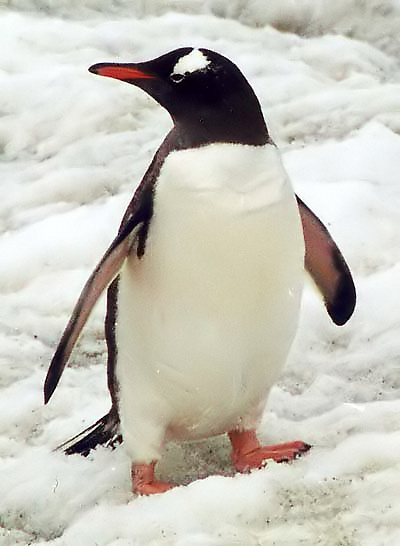
\includegraphics[height=5cm]{figs/penguin.jpg}
    \end{frame}

    \begin{frame}\frametitle{Table}
      \begin{itemize}
        \item How to include tables
      \end{itemize}
      \begin{tabular}{|c|c|c|}
        \hline
        a & b & c \\
        \hline
        aa & bb & cc \\
        aaa & bbb & ccc \\
        \hline
      \end{tabular}
    \end{frame}
  
    % stop page counting for total
    \beginbackup
  
    \begin{frame}[plain]
      \vfill
      \huge{\bf [Backup Slides]}
      \vfill
    \end{frame}
  
    \begin{frame}\frametitle{First slide of backup material}
      \begin{itemize}
        \item First item
        \item Second item
      \end{itemize}
    \end{frame}
    
    % finish backup
    \backupend

\end{document}
